\documentclass[11pt]{article}

\usepackage{amssymb}
\usepackage{amsmath}
\usepackage{dsfont}
\usepackage{graphicx}
\usepackage{multirow}
\usepackage{hyperref}
\usepackage{color}
\usepackage{aas_macros}

\addtolength{\hoffset}{-2.5cm}
\addtolength{\textwidth}{4.5cm}
\addtolength{\voffset}{-2cm}
\addtolength{\textheight}{4.5cm}

\title{Sampling the cosmological parameter space}
\author{}
\date{}

\begin{document}

\maketitle

\section*{The problem}
The target of this work is to get an even sampling of the cosmological parameter space in which points are as spread as possible, within some range; our first application is getting an even sampling of the $(\Omega_m,w,\sigma_8)$ parameter space. To do this we use a similar procedure as \cite{coyote2} and reduce ourselves to the following problem: we want to draw $N$ sample points $\mathbf{x}$ in a $D$ dimensional hypercube of unit side ($\mathbf{x}\in[0,1]^D$) so that the points are as spread as possible. We also want to enforce the \textit{latin hypercube} structure: when projecting the sample on each dimension, the projected points must not overlap. 

\section*{The cost function}
To solve this problem we adopt an optimization approach, in which we define a measure of how "spread" the points are; given a set of $N$ points (or a \textit{design} to use the same terminology as \cite{coyote2}) $\mathcal{D}$, one can define a \textit{cost} function $d_{(p,\lambda)}(\mathcal{D})$

\begin{equation}
\label{cost}
d_{(p,\lambda)}(\mathcal{D}) = \left(\frac{2}{N(N-1)}\sum_{i<j}\left[\frac{D^{1/p}}{\rho_p(\mathbf{x}_i,\mathbf{x}_j)}\right]^\lambda\right)^{1/\lambda}
\end{equation}
%
and $\rho_p$ is just the $p$-distance between two points
\begin{equation}
\label{pdistance}
\rho_p(\mathbf{x}_i,\mathbf{x}_j)=\left[\sum_{d=1}^D\left\vert x_i^d-x_j^d\right\vert^p\right]^{1/p}
\end{equation}
%
What we want is find a design $\mathcal{D}$ that minimizes (\ref{cost}) maintaining the latin hypercube structure. To get an intuition of what's the meaning of this, for $(D,p,\lambda)=(3,2,1)$ this problem is equivalent to the one of minimizing the potential energy of $N$ unit point charges confined in a cube: the repulsive Coulomb force will make sure that these charges are as spread apart as possible. 

\section*{The algorithm}
We use a rough approximation of the simulated annealing algorithm to perform this task: remember that we want to find a latin hypercube design that minimizes (\ref{cost}); the simplest latin hypercube one can think about is a completely diagonal one, call it $\mathcal{D}_0$, defined by the points $x_i^d\equiv i/(N-1)$, $i=0...N-1$, for which one can compute the cost function (which will not depend on $p$, try to believe)
\begin{equation}
\label{diagonalcost}
d_0(N,\lambda) = \left(\frac{2(N-1)^{\lambda-1}}{N}\sum_{i<j}\frac{1}{\vert i-j\vert^\lambda}\right)^{1/\lambda}
\end{equation}
%
This design of course is far from optimal, but we can improve it by shuffling the particles coordinates for each dimension independently, this will greatly improve the cost of the design. What we can do next is exchange the single coordinates of particle pairs and see if this leads to a cost improvement or not: we can iterate this procedure many times to fine tune to the optimum. In detail the algorithm that we use consists in the following steps:
\begin{enumerate}
\item Start from the diagonal design $\mathcal{D}_0$: $x_i^d\equiv i/(N-1)$
\item Shuffle the coordinates of the particles in each dimension independently $x_i^d = \mathcal{P}_d\left(\frac{1}{N-1},\frac{2}{N-1},...,1\right)$ where $\mathcal{P}_1,...,\mathcal{P}_D$ are random independent permutations of $(1,2,...,N)$
\item Pick a random particle pair $(i,j)$ and a random coordinate $d\in\{1,...,D\}$ and swap $x_i^d\leftrightarrow x_j^d$
\item Compute the new cost function, if this is less than the previous step, keep the exchange, otherwise revert the coordinate swap
\item Repeat steps 3 and 4 
\end{enumerate}
%
we found that $10^5$ iterations are enough to achieve convergence (to at least a local optimum) for $N=100$ points in $D=3$ dimensions with the "Coulomb" cost function with $p=2$ and $\lambda=1$.  

\section*{Results}
Using $(N,D,p,\lambda)=(100,3,2,1)$ we computed the cost of the diagonal design $d_0(100,1)\approx8.4$ and we repeated our simplified algorithm for 10 different choices of the random seed required for the random steps in the procedure. The results are shown in Figure \ref{costfig}, which shows a good degree of convergence to an optimum which is independent of the random seed used. Note that the the first random shuffle of the coordinates already knocks down the cost from $\sim$8 to $\sim$3. 
%
\begin{figure}
\begin{center}
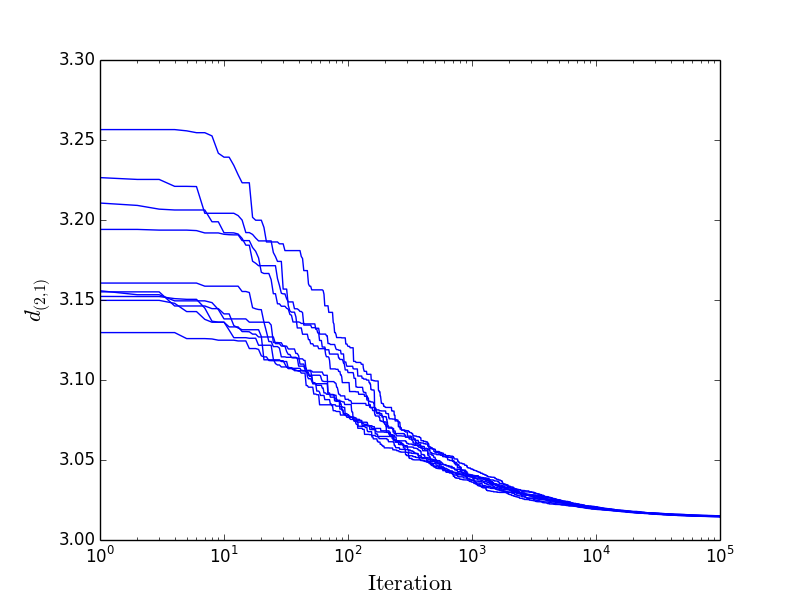
\includegraphics[scale=0.6]{Figures/cost.png}
\end{center}
\caption{Cost function calculated as in (\ref{cost}) as a function of the iteration step for 10 different random seeds}
\label{costfig}
\end{figure}
%
Figure \ref{3Ddistr} show the 3D distribution of points scaled to the $(\Omega_m,w,\sigma_8)$ space in the diagonal configuration, after the first random shuffle and at the found optimum. Figure \ref{2Dproj} shows the analogous 2D projections. 
%
\begin{figure}
\begin{center}
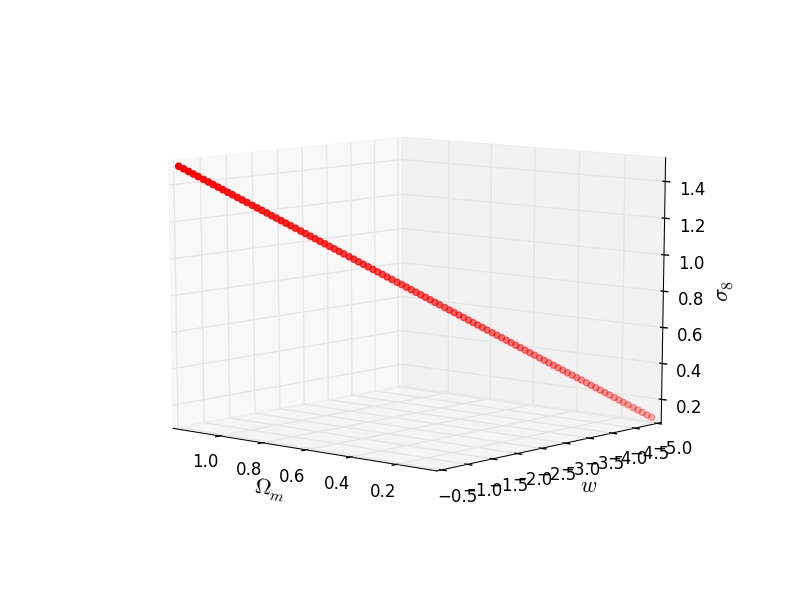
\includegraphics[scale=0.4]{Figures/3dpoints_diagonal.png}
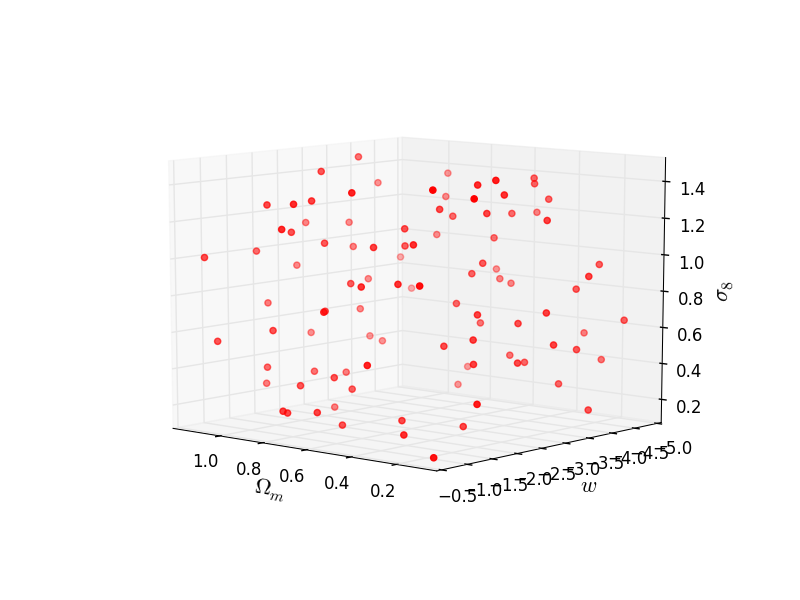
\includegraphics[scale=0.4]{Figures/3dpoints_first_shuffle.png}
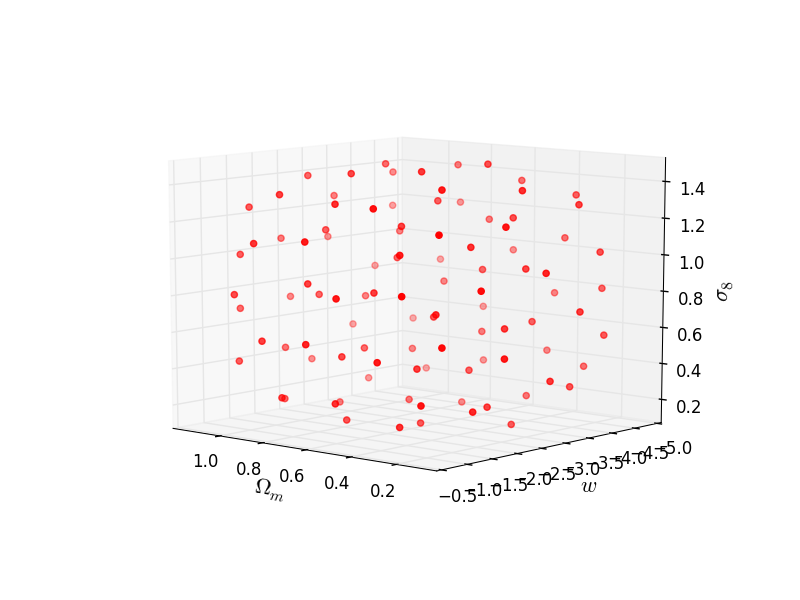
\includegraphics[scale=0.4]{Figures/3dpoints.png}
\end{center}
\caption{Three dimensional distrubution of parameter values at the initial step (top left), after the first random shuffle (top right) and at the optimum (bottom)}
\label{3Ddistr}
\end{figure}
%
\begin{figure}
\begin{center}
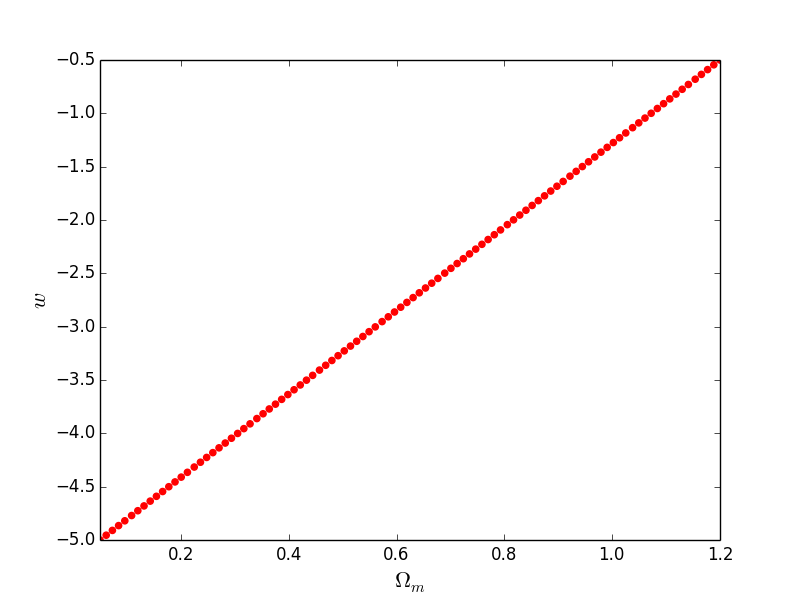
\includegraphics[scale=0.25]{Figures/diag1.png}
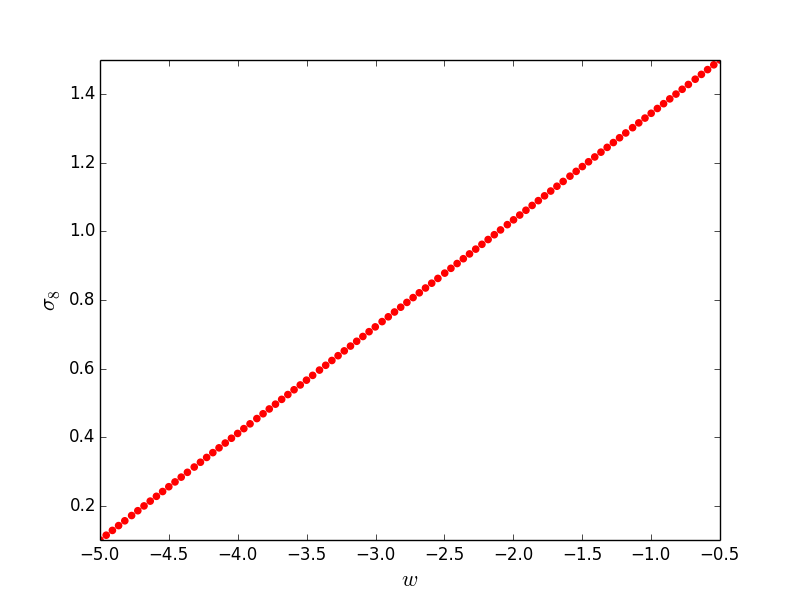
\includegraphics[scale=0.25]{Figures/diag2.png}
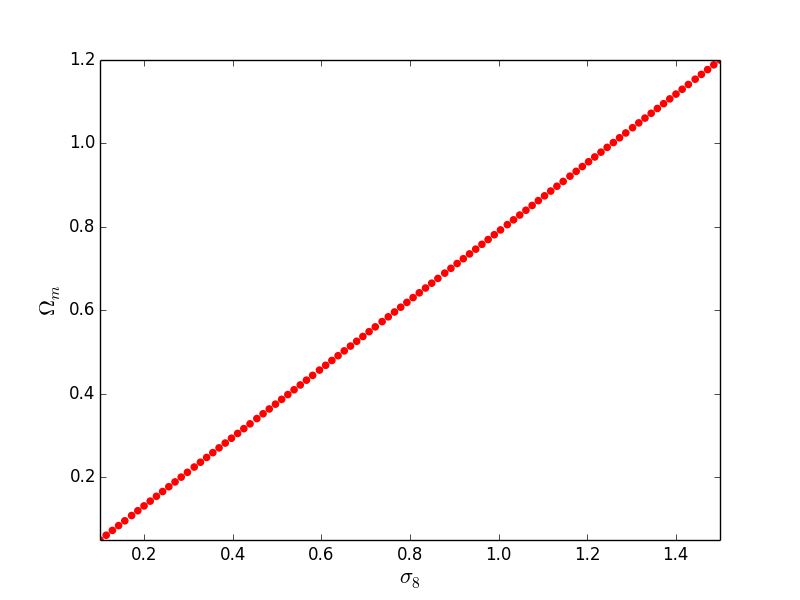
\includegraphics[scale=0.25]{Figures/diag3.png}
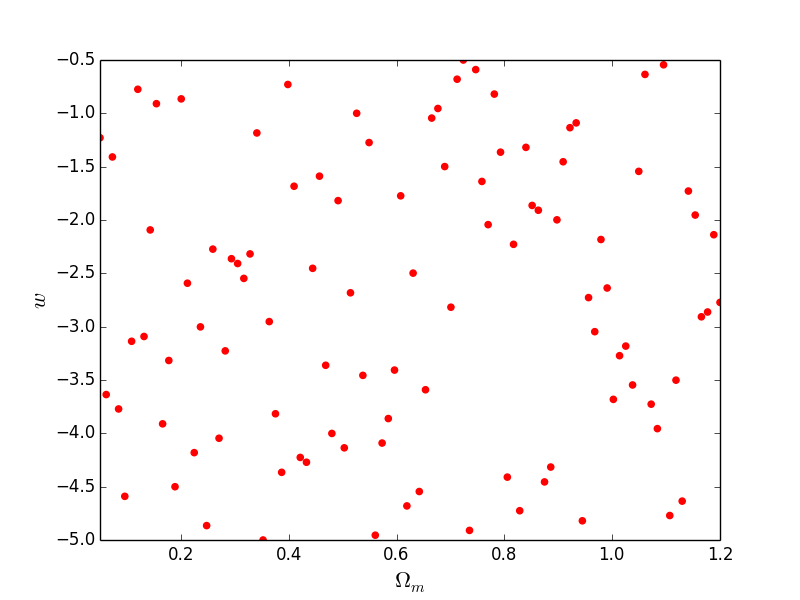
\includegraphics[scale=0.25]{Figures/first_shuffle1.png}
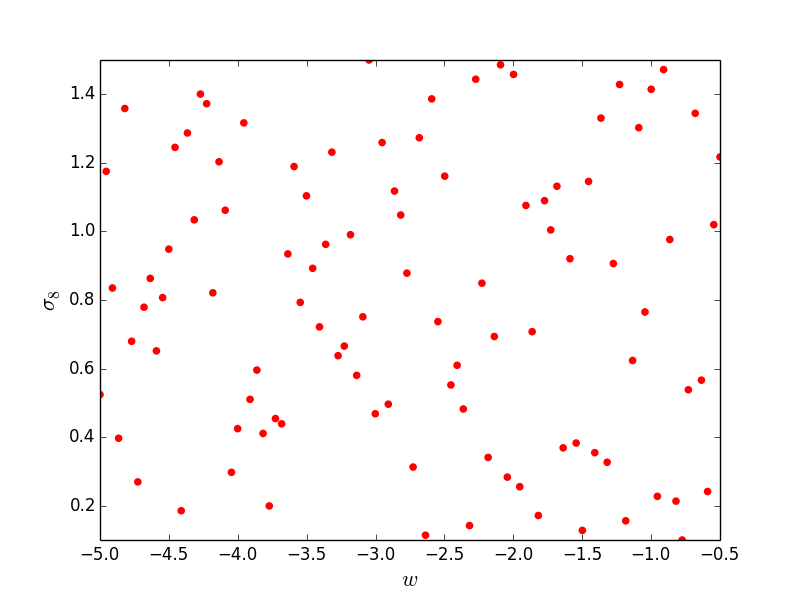
\includegraphics[scale=0.25]{Figures/first_shuffle2.png}
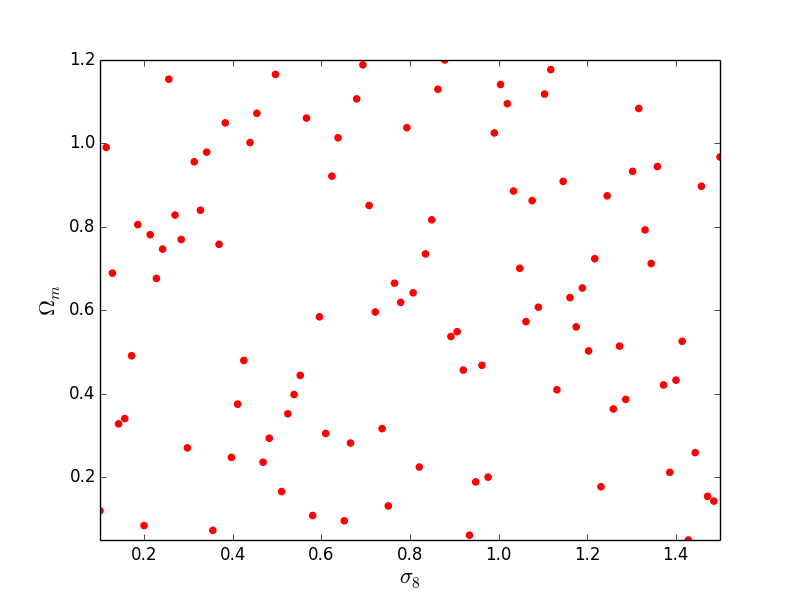
\includegraphics[scale=0.25]{Figures/first_shuffle3.png}
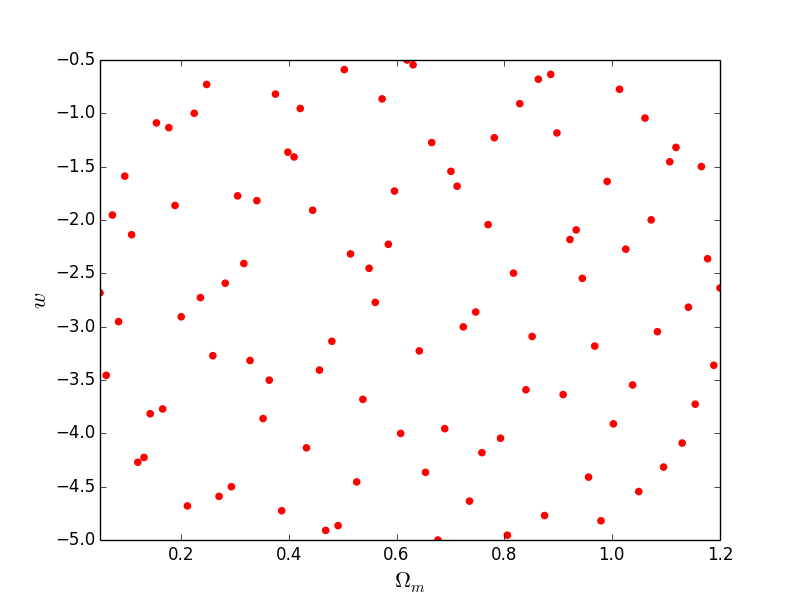
\includegraphics[scale=0.25]{Figures/optimum1.png}
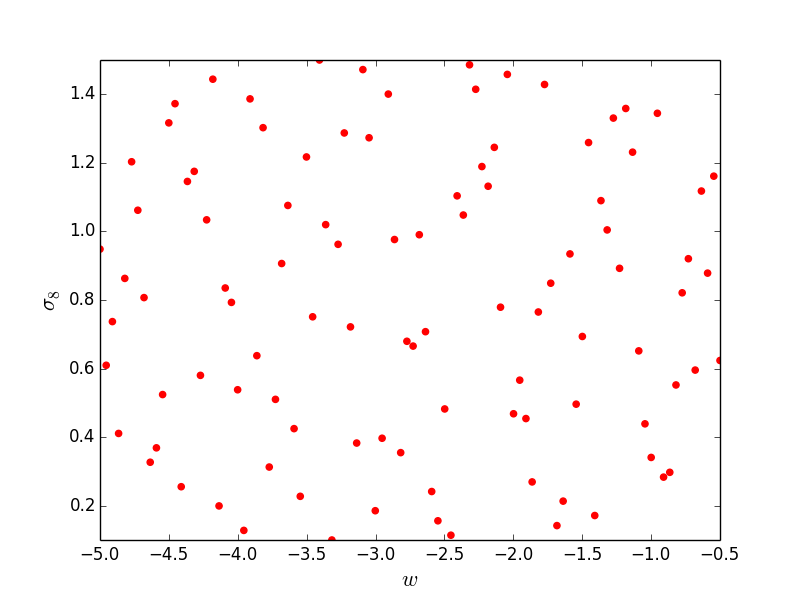
\includegraphics[scale=0.25]{Figures/optimum2.png}
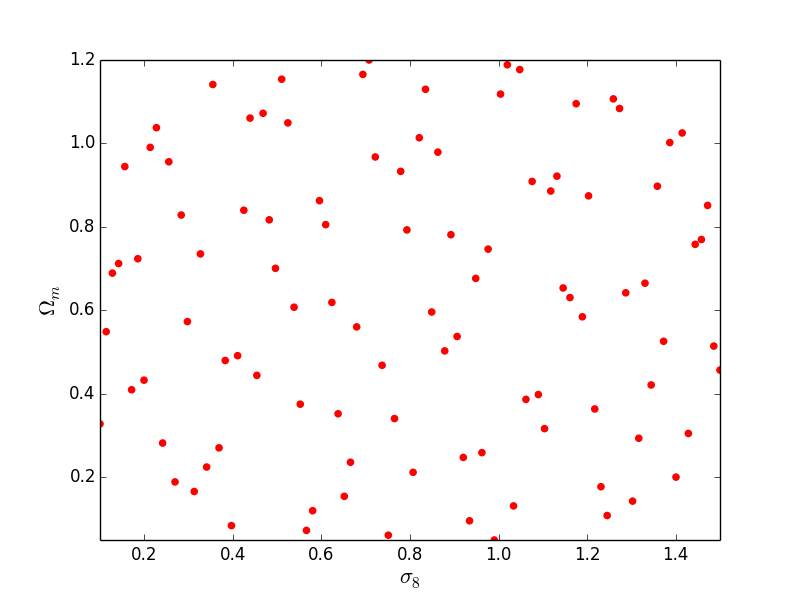
\includegraphics[scale=0.25]{Figures/optimum3.png}
\end{center}
\caption{Two dimensional projections of parameter values at the initial step (top), after the first random shuffle (middle) and at the optimum (bottom)}
\label{2Dproj}
\end{figure} 
%
We can see that the optimization procedure distributes the points in a spherical geometry and gets rid of some of the clumpyness. 
\bibliographystyle{apalike}
\bibliography{ref}

\end{document}